%%%% 
% This is a template for project reports in the subject DAT620 at the
% Department of Electrical Engineering and Computer Science,
% University of Stavanger.
% 
% The template is based on the ACM conference template 
% it was edited by Leander Jehl and Hein Meling
\documentclass[sigconf]{acmart}

%DON'T CHANGE THIS FILE
%This file sets several properties for the ACM template.
%It is not necessary to change this file.


% Copyright
\setcopyright{none}

% DOI
\acmDOI{}

% ISBN
\acmISBN{}

%Conference
\acmConference[Project in Data-intensive Systems (DAT500)]{}{IDE}{UiS}
\acmBooktitle{}
\copyrightyear{2020}

\newcommand{\supervisors}[1]{\thanks{Supervised by #1}}


%In the preamble file you can include packages and define macros.
\usepackage{xspace}

%Here we define a marco: The \xspace ensures correct spacing, i.e. insert space before next word, but not before period or comma.
\newcommand{\paxos}{\textsc{Paxos}\xspace}

%These packages are needed for the plot in Figure 1. 
\usepackage{tikz}
\usepackage{pgfplots}
\pgfplotsset{compat=newest}

\usepackage{listings}
\usepackage{subfigure}

\usepackage{graphicx}
\graphicspath{{fig/}}

\begin{document}
%TODO: Replace the title with your project title.
\title{Search engine for generating a movie cast}
%you may use a subtitle
\subtitle{My project subtitle}

%TODO replace author names with your name and email below:
\author{Christoffer Holmesland}
\affiliation{University of Stavanger, Norway}
\email{cr.holmesland@stud.uis.no}

\author{Malavika Ramakrishnan}
\affiliation{University of Stavanger, Norway}
\email{m.ramakrishnan@stud.uis.no}

%TODO: add the name of one or more supervisors
\supervisors{Leander Jehl and Hein Meling}



\begin{abstract}
%The abstract lies in a different file: 
In this report we show how we used data from IMDB\cite{IMDb} to generate a movie cast based on user input. To determine the 
recommended cast we calculate a score based on genres, actor to actor relationship, and a brief movie summary. The user
is presented with a list of actors and the predicted IMDB user rating score.
\end{abstract}

%TODO: Replace with some keywords, relevant for your project
\keywords{Hadoop, Spark, Film, Casting, Search engine}

\maketitle

%Each section can be placed in a separate file and included by the input command.

\section{Introduction}
\label{sec:introduction}

\noindent
The introduction is different from the abstract; it should elaborate
more on the context of the work and other aspects. Generally, you can repeat some
of the main points also in the introduction, but expand and use different words.

To make your report easier to read, we recommend that you write in first person,
plural, i.e.~write \textit{we}, even if the report is single author.
This is also to represent that, even though you are writing this on your own,
your supervisor and possibly others are contributing ideas, suggestions and
corrections on your report.

What follows is a possible structure of the introduction.
Note that the structure can be modified, but the content should be the same.
Introduction and Abstract should fill at most the first page.

\paragraph{Context and Motivation} The first few sentences in the introduction
is typically a brief description providing context for your work, explaining
the broader domain of the work. This context should lead into the motivation for
the work by identifying one or more problems. 

Here is an example from~\cite{zorfu}:

\textit{Traditional desktop applications, such as word processing, email, and photo management are increasingly moving to server-based deployments. However, moving applications to the cloud can reduce availability because Internet path availability averages only two-nines~\cite{internetPaths}. If a user's application state is isolated on a single server, the availability for that user is limited by the path availability between the user's desktop and that server. Hence, to improve availability, application state must be replicated across multiple servers placed in geographically distributed data centers.}

\paragraph{Research Problem} This paragraph further restricts the problem introduced in the motivation to the problem you are addressing. 
Make sure to explain to the reader 
what you are doing, why it is important, and why it is non-trivial.

\paragraph{Related Work} Next, you have to give a brief overview
of related work. For a paper like this, anywhere between 2
and 8 references. Briefly explain what they do. End the paragraph by
contrasting their work to what you do, to make it precisely clear what
your contribution is.

\paragraph{Contribution Summary} 
It can be a good idea to end the introduction with a summary of your contributions as bullet points.
For example:
\begin{itemize}
\item We implement \paxos using brand new technologies.
\item We evaluate our implementation both in a WAN and LAN environment and show that it is $1.0001\times$ faster than state of the art.
\end{itemize}
It is not necessary to have a paragraph at the end of the introduction, that lists the following sections. 


\section{Related work}
\label{sec:relatedwork}
%!TEX root = main.tex

The IMDB datasets have been used to predict the gross movie revenue\cite{JaeHuang}. The accuracy of several machine learning models were compared to find the best way of predicting the gross revenue. The results show that the random forest model had the best performance and that the most important feature is the number of user votes. The datasets have also been used to compare the user rating with.other features\cite{MaxWoolf}.

In the same analysis they found that lead actors are typically ten years older than lead actresses. The movie project system cinelytic developed by Cinelytic, Inc.\cite{Cinelytic} is able to analyse and produce forecasts of how well a movie will perform based on country, cast and distributor. It also provides useful insights to optimize their content development, financing, production, and distribution decisions. The system ranks actors based on the predicted economic increase they have for a given project. They have partnered with multiple data sources like Netflix, google, the movieDB, Youtube, etc to gather various features relating to a movie.

Our system is similar to cinelytic, but we are basing the score only on IMDB data and use a small subset of the features considered by cinelytic.

\section{Background}
\label{sec:background}
Give a short, self-contained summary of necessary background
information. 

For our example if your project is a new \paxos implementation, the background
would be a brief introduction to the consensus problem, the \paxos algorithm,
the system model used by the \paxos algorithm
and common optimizations and relevant variations of that algorithm.

The goal of the background section is to make the paper 
self-contained for an audience as large as possible. As in every
section you start with a very brief overview of the section.
For our example that would be: In this section, we introduce the consensus problem,
the \paxos algorithm and common optimizations of that algorithm.

If you copy a definition from a text book or some other source, you must cite that source. 
See Example~\ref{def:consensus} below. 

\section{Hadoop cluster}
\label{sec:hadoop}
Our Hadoop cluster consists of one name node and three slave nodes.
The name node has 8 GB RAM and a 2.4 GHz Intel Skylake processor with 4 cores.
The three slave nodes have 4 GB RAM each and a 2.4 GHz Intel Skylake processor with 2 cores.
We used Hadoop version 3.2.1, Spark version 3.0.0-preview2 and Python version 3.5.2.
\\
The Spark documentation recommends using at least 8 GB memory and between 8-16 cores on each node\cite{SparkHardware}. Because our cluster does not meet those requirements, we had to make some changes to the configuration files. We are running the project as a YARN job and we had to keep in mind that the maximum amount of memory configured in YARN had to be greater than what we configure in Spark. It is not recommended to use more than 75\% of the available memory so we decided on 3 GB. The initial amount of memory Spark uses on startup is defined in the spark.driver.memory. The default value is 1GB which we noticed was a bit too much for our cluster. Instead we used 512MB. The Spark driver only runs if we are running Spark in cluster mode. If Spark runs in client mode, the value specified in spark.yarn.am.memory is used instead so this was set to 512MB as well. 

The other Spark configuration value we had to set is spark.executor.memory. This is the memory available to each executor on the worker nodes. When deciding on the value, it is important to keep in mind that there is a default overhead of 7\%, and that the Java virtual machines also require some memory to run. The minimum value of the 7\% overhead is 384MB\cite{SparkOverhead} which means that the value we choose and the overhead had to be lower than the 3GB limit. To be sure that there was enough memory we decided on a spark.executor.memory value of 1512MB.

\section{Your Method}
\label{sec:method}
%!TEX root = main.tex

\subsection{Data collection}

Acquiring the required data for this project in itself was quite challenging. A part the data can be downloaded from the IMDb website\cite{IMDbInterfaces}. This data does not include actor gender, movie plot or box office values. To determine the gender, we used the list of known professions for every person. If they are known for being an actor, they are assigned the label "0", representing male. Actresses are assigned the label "1", representing female. Some people in the dataset have never acted, for example directors or producers. They are removed from the data. There is no way to find the movie plot in the datasets, so we had to find an external source. One alternative is to use webscraping on the IMDB website. We tried doing this but quickly realized that it would not be possible for us to wescrape all the movie plots, because they stop responding to requests after a particular limit in a given time period. We were able to get about 9,000 requests per hour. Since the dataset includes about 500,000 movies, this was not a good solution. It was also not possible for us to know if there were other rate limits e.g. 50,000 requests per day. Instead we used the OMDb API\cite{OMDb} to retrieve the movie plots. Using this API, we were able to get all the plots in 1 hour and 43 minutes. Our original idea was to also make a prediction on the box office value. After using the OMDb API to also find the box office values we saw that only 6381 movies have this value. We do not believe this is enough data to make proper predictions, so we did not use this data. Instead we decided to generate a prediction for the IMDb user score because this value is available for all the movies in our dataset.

One notable challenge was that the data from IMDb is updated every day with new information. This means that you might not get the same result from the search engine as we did when you perform a search. We downloaded the data several times but at one point we noticed that the data can be corrupted, i.e. a lot of information was missing. There seems to be some "luck" involved in the download process. Some days none of the actors have birth years which means that the search engine will not work, other days the ratings were missing. To get the results in this report we used the version of data from the 6th of March 2020. The data from OMDb was only downloaded once on the 12th of March 2020.


\subsection{Preprocessing}

The data from IMDb includes a lot of information we don’t need and it also has missing values. It is also split over several files, e.g. \textit{title.basics.tsv} and \textit{title.ratings.tsv}. Every person in the dataset has a unique id, name, birthyear, deathyear, a list of primary professions and a list of titles they are known for working on. We replace the primary profession list with a number indicating the gender. We remove people who are dead or who has never been an actor or actress before. There are also some people who are actors but not known for any titles. They are also removed because we need that information to calculate a score. These steps reduce the number of people from 9.9 million to 200 thousand.

The data in the \textit{title.basics.tsv} file is an id, type, well known title, original title, adult, start year, end year, runtime, and a list of genres. The only relevant information for our project is the id, type and list of genres. The type is used to decide if we should keep it. We are only interested in looking at movies, represented by "movie" or "tvMovie" in the data. Shorts are typically news segments which would not be a good indicator of movie performance. If we included tv series then the actors in them would have inflated scores because there could be over 100 episodes for a given series. That would show that the person is good at that specific role, but not represent how well he or she can adapt to a new role. The runtime is not used in our system because it is missing for most of the titles. Some movies are missing the genre list and are thus removed because it is a mandatorily required for the system. This reduces the number of titles from 6.5 million to 580 thousand. This might seem like a lot, but most of it is because the data includes separate entries for each season and episode for every TV series. In this step we also use the plot data from the OMDb API. Movies without the plot information are removed. This reduces the number further to 212 thousand.

The movie ratings are in the \textit{title.ratings.tsv} file from IMDB. The format is id, average rating and number of votes. Any title removed from \textit{title.basics.tsv} is also removed from this data. The \textit{title.principals.tsv} file contains a list of the most important people for each title. The fields are title id, ordering, actor id, category, job, characters. We use this information to determine what actors have worked together. We only look at the titles with id which was not removed in the previous step, and the ordering, category, job and characters fields are dropped because they provide no relevant information to us.


\subsection{Ranking algorithm}

The ranking algorithm is used to give a score to the actor groups. The score is given as a number between 0 and 10, where a higher score indicates a higher rank. The final score is a combination of three scores. We call the first one the genre score. It is calculated based on the actors previous performance in that particular genre. The second score is the similarity score. It is calculated from the plot summary of the movies a person has acted in. The third and final score is the relation score between the actor and the other actors in the group. The final score is the average of these scores.


\subsubsection{Genre score}

To calculate the genre score we need to convert the movie data to a different format. The raw data we use are the ratings, principals and title files. They are read by a MRJob script which calculates the weighted average for each genre for each actor. The weights are the number of votes for that title. If an actor has acted in two movies, one with the genres "Adventure" and "Drama", the other with the genres "Adventure" and "Action" then the actor will have genre scores for the genres "Adventure", "Drama" and "Action". The "Drama" and "Action" scores will be the rating that those movies have on IMDb. The "Adventure" score will be a weighted average of both ratings. Assuming that the first movie had 10 votes and a rating of 9, and that the second movie had 90 votes and a rating of 3 then the "Adventure" score is $\frac{10}{10+90}\cdot9+\frac{90}{10+90}\cdot3=3.6$.

Our initial version of the genre score did not consider the number of votes. We quickly realised that a lot of movies have very few votes, and that those movies often have a high rating. It would be hard to set a threshold of minimum number of votes because it could exclude new actors who might not have a lot of experience.

The MRJob consists of one mapper and two reducers. The mapper reads each line and yields the data such that when reducing all of the information for a movie is available on the same line. An example of what is returned if the input line belongs to ratings.tsv is showed in code listing \ref{GenreScoreCode1}. In the first reducer the format is changed from being all of the information about a movie to yielding the information relative to the actor. If for example there are three actors in a movie, then there will be three yield calls with the genres and the rating of the movie. This is shown in code listing \ref{GenreScoreCode2}. The final reducer operates on the actor information and calculates the weighted average of the scores.
\begin{lstlisting}[language=Python, caption=Genre score mapper, label=GenreScoreCode1, breaklines=true]
def mapper_collect_title(self, _, line):
    values = line.split("\t")
    if len(values) == 3:
        yield values[0], ["rating", (values[1], values[2])]
\end{lstlisting}
\begin{lstlisting}[language=Python, caption=Genre score first reducer, label=GenreScoreCode2, breaklines=true]
def reducer_title(self, key, values):
    # Generation of the genres object omitted.
    genre_ratings = {genre: rating for genre in genres}
    for value in values:
        if value[0] == "actor":
            yield value[1], genre_ratings
\end{lstlisting}

\subsubsection{Similarity score}
The similarity score is calculated by comparing the summary plot given as input by the user and the summary of the movies acted by the actors with high genre scores. For this purpose, we tried the following methods:

\begin{itemize}
    \item \textbf{Cosine similarity using Tf-idf:}The cosine similarity is the cosine of the angle between two vectors. In text analysis, each document can be represented as a vector. Mathematically, cosine is the dot/scalar product of two vectors divided by the product of their Euclidean norms. The lesser the value of cosine, the lesser the similarity between the two documents and vice versa. Tf-idf is short for term frequency-inverse document frequency and is often used in information retrieval and text mining. The text in the documents are tokenized and lemmatised, then tf-idf measures the frequency of each word occurring in a document, and comes up with a tf-idf matrix whose similarity is then computed. This method depends very much on the number of words in a document. Which is why this was a bad choice for our task, since our plot summaries are small, with very few words. Nevertheless, we tried implementing this, but the results were highly dissatisfactory.    
    \item \textbf{Word2Vec: }Word2Vec as the name sounds is a neural network that maps words to a vector and then analyses them mathematically. Its purpose is to cluster the vectors of similar words together in a vector space. That is, it detects similarities mathematically. Word2vec creates vectors that are distributed numerical representations of word features, features such as the context of individual words. This  method  was  highly  promising  but  yielded  poor  results since it was computing word-wise similarity while we needed sentence-synonymity.
    \item \textbf{Tensorflow model from Google: }The model \cite{TFHubModel} available in the TensorFlow Hub is also a form of word2vec model but is instead trained and optimized for greater-than-word length text, such as sentences, phrases or short paragraphs. This perfectly matched our criteria and gave excellent results. This model would return a value between 0 and 1 which we multiplied by 10 to normalise it like the genre score.
\end{itemize}

There is a large drawback to using a tensorflow model when the program runs on Spark. The model is quite large, almost one gigabyte. Usually a spark broadcast variable would be used to share an object between nodes but in this case it couldn’t be done because the model cannot be pickled which is a requirement for broadcast variables. To be able to use it on the slaves each of them would have to load it into memory instead. To achieve this we defined closures for each partition of the data where the tensorflow library was imported and the model was loaded. Importing the tensorflow library is quite expensive. It usually halts for 30 seconds before the import is done. Loading the model is equally expensive, thus the total time on each partition is a minute before work can start. Because there is multiple partitions per node, the model is loaded several times on each of them. In our case this took so much time that the algorithm hadn’t finished after several hours. We didn’t consider this acceptable and looked for a different alterantive. The best solution we found was to do the calculations on the master node instead. Because it has more memory available, we were able to load the model once and calculate the similarity score for each title using the rdd.toLocalIterator() generator of the DataFrame, shown in code listing \ref{CodeToLocalIterator}. This means that all of the data had to be transferred over the network to the master node, and then back again to the slave nodes when the calculations were done, but this was actually faster in our cluster than the former method. The runtime of similarity score is typically about 8 minutes. The initial version was a bit slower, but when we decided to pre-allocate the lists where the similarity score is stored before being turned into a DataFrame the performance improved. We do however recognize that transferring the data over the network might be a bad option in general and think that if we had more time to work on this we would have looked for a better solution.

\begin{lstlisting}[language=Python, caption=Plot similarity, label=CodeToLocalIterator, breaklines=true]
scores = [None] * movies.count()
sim_arr = [search_plot, None]

# Iterate over every movie summary and calculate the similarity score
for i, row in enumerate(movies.rdd.toLocalIterator()):
    sim_arr[1] = row.summary
    sim = sim_model(sim_arr)
    scores[i] = (row.tconst, 10 * float(np.dot(sim[0], sim[1])))
\end{lstlisting}

\subsubsection{Relation score}

The two previous scores are independent of each actor. We believe this is a good way of measuring the performance of each actor. However, when combining the actors to groups, we wanted to have some measure of how good two actors work together such that the groups were not just the top ranked candidates based on the independent scores but also how well their on-screen combination worked. Our initial idea was to consider the first candidate list as the primary actor, and only include actors from the other candidate lists if they had acted with someone in the primary candidate list previously. This turned out to be a really bad way because there were not that many direct relationships in the data. When looking for alternatives, we found the Spark GraphX framework and got inspired to make a relationship graph instead to achieve the same goal. GraphX cannot be used in PySpark so we had to implement the graph ourselves. The main idea is that if two people have acted together then they have a relationship of strength equal to the IMDB rating of the title they worked on.

The initial version of this was implemented in Python using Pandas dataframes, because we found that the overhead of working on Spark made it harder to explore ideas quickly. The graph was stored in a dataframe where index is the multi-index from\_node, to\_node. The only column is what we call the inverse of the rating. The inverse of the rating is simply ten minus the rating. This is done because it enables us to use an algorithm to find the shortest path between two nodes on the graph. If you are unfamiliar with graph algorithms, we would like you to note that the shortest path doesn’t actually mean as few nodes as possible. The proper description is the path which minimises the cost function between two nodes. The shortest path would be along the lowest numbers, which in turn means along the highest ratings. A graph with the rating itself as the edge cost would require an algorithm which maximises the cost. The maximum cost would be to never arrive at the goal node because the cost could always be increased by simply visiting a different node before visiting the goal node. We decided to implement Dijkstra’s algorithm to find the path between two nodes. It finds the path by looking at the edges from the starting node, picking the one with the lowest cost and then looking at that node’s edges. This continues until the goal node is found, see code listing \ref{CodeDijkstra}. Because we always look at the node with the lowest cost, we can be sure that the path to the goal node actually is the shortest path. The original version of the algorithm works on two nodes at a time, but there exist variants that can find the path between one node and every other node.

\begin{lstlisting}[language=Python, caption=Dijkstra pseudocode, label=CodeDijkstra, breaklines=true]
queue = [start_node]
while len(queue) > 0:
    current = queue.get_lowest_cost_node()
    if current == goal:
        return score, path
    for edge in current.edges:
        edge.set_score()
        if edge in queue:
            queue.try_update_score(edge)
        else:
            queue.add(edge)
\end{lstlisting}

Dijkstra's algorithm works great when all of the data is in memory like it is when it is stored in a Pandas dataframe. It is quite slow to execute because of the size of our data. The graph consists of almost one million nodes, and between 10 and 350 edges from each node. The execution depends on the nodes we are finding the path between but in general the time is about 20 minutes. When we moved over to the Spark version of the algorithm, we kept this in mind. Let us first make some assumptions. If we take the top 30 candidates from each candidate list, and there are three candidate lists, then we need to calculate 3· $(30*30)=2700$ relationship scores. If each of them needs 20 minutes to finish, then the execution time would not be acceptable. Even if each score was calculated in just one second the total time would be 45 minutes. When we implemented Dijkstra's algorithm on Spark, the runtime was even worse because each step requires that some data is transferred from a slave to the master and then back again. Because of the way Dijkstra's algorithm works, state has to be shared between each worker, and thus data has to travel over the network. To avoid this, we decided to implement our own algorithm instead which doesn’t have that requirement. We tried to find previous work on graph algorithms on Spark, but all of them were using Spark GraphX which we couldn’t do.

Our solution was to create a greedy fixed step algorithm inspired by the breadth first algorithm. The breadth first algorithm simply looks at all of the edges for a node before continuing. The reason for making it a greedy fixed step algorithm is the challenge which is the size of our graph. As an example, you can start at Leonardo DiCaprio and look at the number of edges. In our graph he is connected to 350 other actors. It would be really quick to calculate the shortest path if the goal actor were directly connected to Leonardo. For most relationships there is not a direct connection, and so we have to also look at the edges of each edge. This increases the number of paths to 58,339 which isn’t that many considering the size of the graph. If the goal is still not found the number of paths is increased again by looking at the edges of the edges to 8,901,575. If we again assume 2700 relationships, then the number of paths to check is over 24 billion. This is doable but it does increase the execution time a lot. If the relationship isn’t found in those 8.9 million paths, then another step outward can be taken to increase the number of paths to 1.3 billion. This would be a total of 3.5 trillion different paths which is so large that the execution time would not be acceptable. We therefore decided that the fixed step should be either 2 or 3. This also makes sense at a conceptual level. If you consider the relationship between two actors A and B. If A worked with C and C worked with B, then it makes sense to say that their working relationship is important. The same can be said about the relationship A-C-D-B which is a 3-step relationship. If the relationship is more distant, it makes sense to value it lower than a close relationship. This caused us to change the cost function between two nodes. Instead of being just the inverse of the rating, it was changed to be the average of the inverse distance and the inverse rating. The combination of the 2 or 3 step algorithm and the new cost function means that only the close relationships will affect the group score. A close and good relationship increases the score, while a close and bad relationship decreases the score. Any distant, meaning greater than 2 or 3 steps, will not change the score.

\begin{figure}[t]
    \centering
    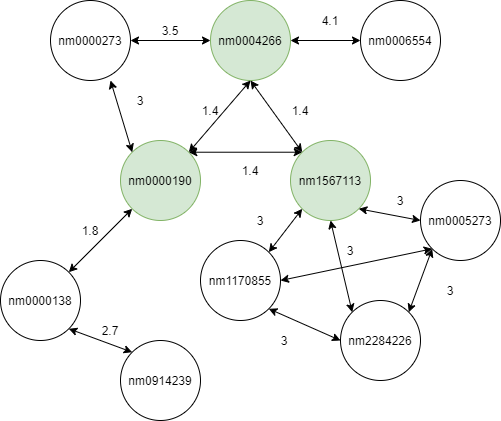
\includegraphics[width=\linewidth]{relation_graph.png}
    \justifying
    \small
    For the Use case example (Interstellar): Matthew McConaughey: nm0000190, Anne Hathaway: nm0004266, Jessica Chastain: nm1567113 are the main actors. The edges represent the average of the inverse distance and the inverse rating.
    \caption{A sample snapshot of the actor-actor relationship graph}
\end{figure}

Since we have not been able to find a description of a multi start and end node breadth first algorithm we would like to include a description of it. The first iteration of our algorithm is the normal breadth first algorithm. The graph is stored in a DataFrame, and the current paths are stored in another DataFrame. Start by taking the starting node and adding it and every edge from it to the DataFrame. Continue adding edges to the DataFrame n times, where n is the number of steps you are using. The resulting DataFrame should have several columns where the first one is the starting node, the following columns should be the edge and cost to that edge. By applying a function to each row of the DataFrame we can calculate the cost from the starting node to the last edge node following the path along every edge in that row. If the goal node is found along the path, then we return the cost, otherwise a token value is returned. The token value should be outside of the cost function domain or be on an extreme of the domain meaning that in any situation it will not be considered as a possible path to the goal node. In our case, we use a token value of -1 because the domain of our cost function is [0, 10]. The inverse of the cost function is returned and stored in a score column. Finally, the score column is aggregated to find the maximum and this is returned as the relation score between the two actor nodes. By observing that calculating the path from A-B-C is done by a 2-step search from A, is done no matter what our goal node is. The algorithm can be improved by allowing a list of goal nodes. When applying the cost function simply check if any of the goal nodes are found along the path. This is a simple change that improves the exeuction time a lot. If you look at the score between one actor and 8 other actors, the exeuction time is about 20 seconds for each relation if you are using the breadth first algorithm. With the multi goal optimisation, the time is reduced to about 2.5 seconds for each relation. When calculating the relation scores between the candidate lists A and B of size 30 each, the number of function calls is now reduced from 90 to just 30. A simplified version of this function is shown in code listing \ref{CodeBFS}.

\begin{lstlisting}[language=Python, caption=Simplified multi-start to multi-goal search algorithm, label=CodeBFS, breaklines=true]
# Get initial nodes and their edges
current = graph.filter(F.col("node").isin(start_nodes))
current = current.join(graph, current.node == graph.node)
# Do n steps
for i in range(1, n):
    current = current.select("*", F.explode(current.edges))
    current = current.join(graph, current.last_node == graph.node)
# Split by starting node and find best score
current = current.withColumn("score", calculate_score(current.columns))
current = current.select("start", F.explode(F.col("score")).alias("goal", "score"))
best_scores = current.groupby(["start", "goal"]).max("score").collect()
return best_scores
\end{lstlisting}

By observing that the same calculations are done when finding the path from A1 to B and A2 to B we can improve it further to a multi start node algorithm. The most expensive part of the algorithm is transferring the graph edges to the current path. The number of times we do this grows with the number of times we call the merge function on two dataframes. By looking at the path from multiple start nodes to multiple goal nodes the number of merges is reduced and the number of function calls can be reduced to 1. 

Following the assumptions from before, the total time for a 2-step search is 129 seconds. This gives a time per relation of 0.048 seconds which means that compared to the original algorithm, the execution time has been improved by a factor of 9500. The number of paths for the 3-step search is quite a bit larger but the improvement is still significant. The total execution time is 4402 seconds, giving a time per relation of 1.63 seconds which is a 280 times improvement. 

\subsubsection{Overall score}

The ranking algorithm is used to determine whether one actor could perform better than another. This is done by calculating a score for the actors, before combining them to get a score for the whole group. Our algorithm assumes the first actor description to be the primary actor and tries to maximise the cast rank based on this. The following is a description of our algorithm. The first step is to find every actor that matches the primary actor description. For every matching actor, a score is calculated. It is a combination of the genre score, past acting relationship (maybe) and how similar the plots of the movies the actor has acted in are to the user plot. The genre score is taken as the average of the actor genre scores, given that they match the user genres. This is done because one actor might have a high score in war and action movies, but low in romance and drama. If the user is making a romance and drama movie, then the genre score is taken as the average of just those two scores. The plot of every movie the actor has been in is compared to the user plot. The maximum similarity score is used for the actor score. To make the average of the genre score and the similarity equally important for the actor score the similarity bound is changed to (0, 10).Then the actor score is changed to be in the interval (0, 1). Thus the expression for the score is: $actor(id)=\frac{1}{20}(avg(genrescore)+5.(max(similarity)+1))$.To find the other actors the procedure above is repeated on the actors matching the other descriptions. Because we consider it beneficial to cast actors who have worked together before, we use the relation score calculation above stated to calculate the actor relation score. To calculate the cast score, we also make a prediction of the IMDB rating that the resulting movie will have if the selected actors are in it. The prediction is calculated from the average of the actors’ average genre scores. The expression for the cast score is: $cast(ids)=\frac{1}{\#ids}\sum_{i=1}^{\#ids}worked(ids_i, ids_1)\cdot actor(ids_i) + rating(ids)$. The $worked$ function returns X if they have worked together before, 0 otherwise. 

The cast score is used to rank the groups. A higher score means a better group. The groups are sorted in descending order and returned to the user.

\subsection{Workflow}

The summary of the workflow for our project is pictorially represented in the two figures. The Python process is described in figure \ref{PythonWorkflow}, and the Spark process is described in figure \ref{SparkWorkflow}. 

\begin{figure*}[h]
    \centering
    
\includegraphics[width=\textwidth]{workflow.png}
    \caption{Python Process Workflow}
    \label{PythonWorkflow}
\end{figure*}

\begin{figure*}[h]
    \centering
    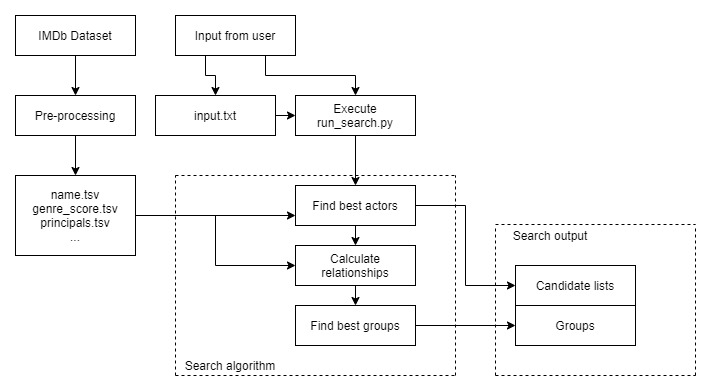
\includegraphics[width=\textwidth]{SparkProcess.jpg}
    \caption{Spark Process Workflow}
    \label{SparkWorkflow}
\end{figure*}

\subsection{Algorithm results}

The runtime of our algorithm is not the only evaluation we need to base our efficiency on. The result of a search is equally or more important. We first need to define what a good result is, and then how we decide whether or not a result is better than another. The obvious answer to what a good result is, is one that maximises the scores discussed in the previous sections. Following from that answer we also need to justify why those are good methods of measuring an actors’ ability to perform well. We think it is intuitively true that if an actor has performed well earlier, they are more likely to perform well in their next movie of the same genre than someone who has a comparatively bad acting history. The same can be said about the similarity score, if someone has acted in a similar movie before then they are likely familiar with the setting and mindset they need to be in while acting. This does not however hold when arguing why the relationship score is relevant. Our reasonable justification for this is that we believe the assumption: "Any movie with a high user rating on IMDb has a good cast" to be true. From this we can say that if two actors have acted together in a movie with a high rating then they are good at acting together, and the opposite if the movie has a low rating then they should probably not act together. This assumption also means that we should have the following goal for our search engine: if you do a search with the attributes from a movie on IMDb, the original cast should be early in the result if the movie has a high rating. There is a fallacy to be aware of here. If you only try to achieve this goal, for example by weighing the similarity score and the relationship score by a large constant, then the individual is lost and the engine will most likely only return previous movie casts for any new query. 

We believe we found a good balance between the importance of the different scores. A problem with the result we discovered while working on the engine is that when combining individual actors into groups then you need to have some measure of their relationship to avoid having the groups be a combination of just the individually best actors. What we mean by this is that if A and B actors have a sufficiently large score then they will be the suggested for several of the top groups, for example ABC, ABD, ABE, ABF and so on. This is of course the correct result based on the score, but it does not give a lot of information to the user because they are suggested a low number of actors relative to the number of groups. E.g. five groups make it possible to have 15 distinct actors, but the actual result might only contain 7 actors if the two first candidates are constant. This problem was our main motivation behind adding the relationship score. While it did help alleviate the problem, we still feel like this is a major problem with our search engine. To improve the result we decided to include the top ranked candidates from each list together with the top groups such that if the user feels like some actors are repeated too often then they can look at the individual lists for other alternatives.


\section{Experimental Evaluation}
\label{sec:evaluation}
%!TEX root = main.tex

In this section, we are going to look at the difference in runtime between the implementation in Python and the Spark implementation. We are also going to show the results of some search queries.



\subsection{Experimental setup}

The MRJob/Spark implementation code ran on the Hadoop cluster described in the Hadoop cluster section. The Python implementation ran on a machine running Windows 10 Pro with the following hardware: Intel i5-8600K 3.6GHz CPU, 16 GB DDR4 2667MHz memory, and a SSD disk with a read speed of 500MB/s and a write speed of 320MB/s. The Python version used is 3.7.4 64-bit. To measure the execution time of the pre-processing scripts we used the time(1)\cite{Time1} linux command. To be able to use linux commands on a Windows machine, we used the Git Bash terminal\cite{GitBash}. In the pre-processing steps each task is implemented in MRJob except the graph task which was implemented in Spark. The algorithm steps are implemented using Spark. The time unit is seconds unless otherwise specified. To measure the execution time, we used the time function from the time library in Python. We were not able to use the time(1) command because we wanted to measure several functions defined in the same script



\subsection{Results}

\subsubsection{Pre-processing}

As shown in the table \ref{tab:preprocess runtime} there is a significant difference between the implementations. The Python implementation is about 3.5 times faster than the implementation running on Hadoop. There are three main reasons for why the difference is so large.
 
The first and most important one is that there is an overhead when you use Hadoop. The time to connect and actually start the job is typically between 45 and 60 seconds. This means that since six tasks are executed the overhead could be as much as 360 seconds which is almost as much as the total time of the Python implementation. 

The second reason for why the Python implementation is faster is because all of the data is able to fit in memory at once, while the Hadoop implementation requires data to be stored on multiple nodes and transferred between them. 

The third reason is because the machine running the Python code is faster, it has more memory and a faster processor. Since the pre-processing is only supposed to happen once, we decided to not spend a lot of time optimizing the code so that we could focus on the algorithm instead.

\begin{table}[H]
\centering
    \begin{tabular}{ |c|c|c| } 
        \hline
        \textbf{Task} & \textbf{Python} & \textbf{MRJob / Spark} \\ 
        \hline
        name\_basics & 25.5 & 102.3 \\ 
        title\_basics & 17.5 & 89.6 \\
        title\_principals & 32.9 & 664.3 \\ 
        title\_ratings & 2.0 & 67.0 \\ 
        graph & 106.6 & 205.3 \\ 
        genre\_score & 195.2 & 232.3 \\ \hline
        \textbf{Total} & \textbf{379.7} & \textbf{1360.8} \\ 
        \hline
    \end{tabular}
    \caption{Pre-processing runtime of Python and Spark in seconds}
    \label{tab:preprocess runtime}
\end{table}

\subsubsection{Algorithm}

The search query execution times were measured while using the attributes from the Interstellar movie. The total Python time is an estimate based on the relation score measurement. The relation score times are reported as a per relation score to better reflect the difference. The reason for why the difference is so great is because the Spark implementation is able to compute multiple relation scores at the same time, while the Python implementation can only compute one at a time. A more detailed explanation of the difference can be found in the Relation score section in part 5. In the execution time of the algorithm we can again see that when transferring data between nodes is required, the time increases a lot. This is why the Python implementation is faster in the candidate actors’ task and the similarity score task. As we discussed in the similarity score section, we were not able to figure out a good method of sharing the tensorflow model between the worker nodes on Spark which is why the time is significantly greater in this task. The relation score time was calculated while running a 2-step search. When the number of steps is increased to three the run time per relation is increased to 0.4 seconds.



\begin{table}[H]
	\centering
    \begin{tabular}{ |c|c|c| } 
        \hline
        \textbf{Task} & \textbf{Python} & \textbf{Spark} \\ 
        \hline
        candidate actors & 60.3 & 331.5 \\ 
        similarity score & 89.6 & 448.8 \\ 
        relation score & 438.0 & 0.0362 \\ \hline
        \textbf{Total} & \textbf{13.7 days} & \textbf{1182.1} \\ 
        \hline
    \end{tabular}
	\caption{Algorithm runtime of Python and Spark in seconds}
	\label{tab:algorithm runtime}
\end{table}



The search query execution times were measured while using the attributes from the Interstellar movie. The total Python time is an estimate based on the relation score measurement. The relation score times are reported as a per relation score to better reflect the difference. The reason for why the difference is so great is because the Spark implementation is able to compute multiple relation scores at the same time, while the Python implementation can only compute one. A more detailed explanation of the difference can be found in the Relation score section in part 5. In the execution time of the algorithm we can again see that when transferring data between nodes is required the time increases a lot. This is why the Python implementation is faster in the candidate actors task and the similarity score task. As we discussed in the similarity score section we were not able to figure out a good method of sharing the tensorflow model between the worker nodes on Spark which is why the time is significantly greater in this task. The relation score time was calculated while running a 2-step search. When the number of steps is increased to three the run time per relation is increased to 0.4 seconds.



\subsubsection{Search result}

The search engine is not limited to five groups for a search query. It will return groups using the top 25 actors from each candidate list, and also return the complete candidate list for each query. A more complete search result is shown in Section \ref{sec:appendixA}, Appendix A - Search result. The following tables are the top five groups from two search queries. It is also possible to have queries where the number of actors is not three. 



\begin{table}[H]
\centering
    \begin{tabular}{ |c|c|c|c| } 
        \hline
        \textbf{Actor 1} & \textbf{Actor 2} & \textbf{Actor 3} & \textbf{Score} \\ 
        \hline
        nm0000190 & nm0004266 & nm1567113  & 9.145267 \\ 
        nm0000190 & nm0544718 & nm1567113  & 8.54046 \\ 
        nm0000354 & nm0004266 & nm1567113  & 8.534471 \\ 
        nm0000190 & nm0004266 & nm1325419  & 8.496985 \\ 
        nm0000190 & nm0004266 & nm0000234  & 8.451193 \\ 
        \hline
    \end{tabular}
	\caption{Interstellar attributes with a 3-step relation score search}
	\label{tab:3-step relation score}
\end{table}



The original actors from the Interstallar movie are Matthew McConaughey: nm0000190, Anne Hathaway: nm0004266, Jessica Chastain: nm1567113. As the result show we achieved our goal of getting the original cast highly ranked by the engine.

However, it also highlights the largest problem we have been struggling to solve, which is that groups often contain the same actors. In this result the original actor from the second candidate list is the recommendation for eight of the top ten groups. The first candidate is repeated less, only four times in the top ten groups.



\begin{table}[H]
	\centering
    \begin{tabular}{ |c|c|c|c| } 
        \hline
        \textbf{Actor 1} & \textbf{Actor 2} & \textbf{Actor 3} & \textbf{Score} \\ 
        \hline
        nm2633535 & nm1126657 & nm1107001  & 6.8459167 \\ 
        nm2633535 & nm1126657 & nm0941777  & 6.8427186 \\ 
        nm3836977 & nm2056274 & nm2356421 & 6.8229513 \\ 
        nm2633535 & nm1126657 & nm1212722  & 6.8178062 \\ 
        nm2633535 & nm1126657 & nm1310016  & 6.790106 \\ 
        \hline
    \end{tabular}
\caption{1917 attributes with a 2-step relation score search}
\label{tab:2-step relation score}
\end{table}



The only original actor present in the result is George MacKay: nm1126657. Our initial thought was that the other actors must not be very good which turned out not to be true because both of them have acted in titles like Game of Thrones and Star Wars. The reason is that their birth year is missing from the data. This means that the engine is not able to consider them as candidates because their age cannot be determined.

\section{Conclusion}
\label {sec:conclusion}
Here you need to summarize what you did and why this is
important. Do not take the abstract and put it in the past
tense. Remember, now the reader has (hopefully) read the
paper, so it is a very different situation from the abstract.
Try to highlight important results and say the things you really
want to get across such as high-level statements (e.g.,
we believe that .... is the right approach to .... Even though
we only considered LAN, the .... technique should be applicable
....) You can also formulate next steps if you want.
Be brief.

\section{Citation}
\label{sec:citation}
It is important that you correctly refer to sources. 

\begin{itemize}
\item If you describe background, according to some textbook, cite that textbook. \emph{See Example~\ref{def:consensus} below.}
\item If you make a claim about trends in industry or research, add citations to validate the claim. \emph{See Example~\ref{ex:trend} below.}
\item \textbf{Do not copy paste text from any source into your report without citation. It will be considered plagiarism.}
\item Always use the tilde character between the text and the cite command, e.g.:\begin{verbatim}
DBLP~\cite{dplg}
\end{verbatim}
The tilde inserts a space, but prevents line break between the text and citation.
\item For correct citations we recommend that you export bibtex entries from DBLP~\cite{dplg}. 
%@Hein: ACM produces crappy doi-urls for non ACM publications. I do believe that there are few papers that are part of the ACM-DL and not in DBLP.
But make sure to update the bibtex entries to adhere to the following rules.
\end{itemize}

Here are some rules to be followed for your bibliography:

\begin{itemize}
\item Make sure titles are correctly capitalized.

%You can export all nsdi citations from DBLP, accordingly this should not be a problem.
% \item Make sure abbreviations are consistent (e.g., is NSDI spelled out or
% not?) - using the @abbrev function in latex helps here.

\item Make sure there is enough info for a reader to find the document: authors
plus title isn't enough.

\item Don't blindly copy and paste ACM bibtex entries without fixing them:

- they list "New York, NY" as the address field, which means that all ACM
conferences look like they took place there; just delete this, or - better

- replace it with where the conference took place, which is much more
helpful to the reader than the publisher's address

- they have a truly weird idea about how to capitalize conference names;
just correct this (consistently)

* IEEE is equally bad, and uses a partially-inverted form of conference
names.

* Please actually review the bibliography before submitting your paper!
\end{itemize}

%@Leander: Move this to the Latex part:

And while you are at it, please:

\begin{itemize}
\item Add include{mathpmtc} in the main LaTeX file, so you don't have
math stuff in a different font than the main text. 
%We could simply add this to the template if not already done.

\item Always use the tilde character between the number and unit, e.g. 100~Mbps or 53~ms. 
The tilde inserts a space, but prevents line break between the number and unit.

\item Never put SI units in italics. 

\item Do differentiate between bits (b) and bytes (B), and between powers of 10~(MB) and 2~(MiB).

\item Avoid things like: "We refer the reader to [42]." That is, don't use citations as nouns.
\end{itemize}


\begin{example}
\label{def:consensus}
Consensus is a distributed programming abstraction that fulfills the following properties~\cite{aTextbook}:
\begin{description}
\item[Termination]
\item[Validity]
\item[Integrity]
\item[Agreement]
\end{description}
\end{example}

\noindent
\begin{example}
\label{ex:trend} Consensus systems build a fundamental part of todays cloud-computing infrastructure~\cite{spanner,chubby,zookeeper,zookeeperWeb}.
\end{example}




\section{Latex}
\label{sec:latex} 
This section contains some instructions and examples for using \LaTeX.

\subsection{You can add subsections}
You can use numbered subsections to structure your sections or $\backslash\texttt{paragraph}$ to separate paragraphs with a heading using only a few words, as used in Section~\ref{sec:introduction}.


\begin{enumerate}
	\item\label{item:1} This is an item in an enumeration.
    \begin{itemize}
    	\item This is an item of a unnumbered list. In this case, the lists are nested within each other.
    \end{itemize}
    \item\label{item:2} The second point in the enumerated list.
\end{enumerate}
%
I can refer to the element of the enumeration above as Point~\ref{item:1}.
If you refer to numbered items,~e.g. items from a list or figures or sections, always capitalize the name. 
For example, this is Section~\ref{sec:latex}.

\subsection{Figures}
You can include figures. You can include files, as done in Figure~\ref{fig:example}. 
Avoid including jpeg, gif or bmp files since these do not scale nicely. Again Figure~\ref{fig:example} is an example for that.

\begin{figure}[t]
   \centering
   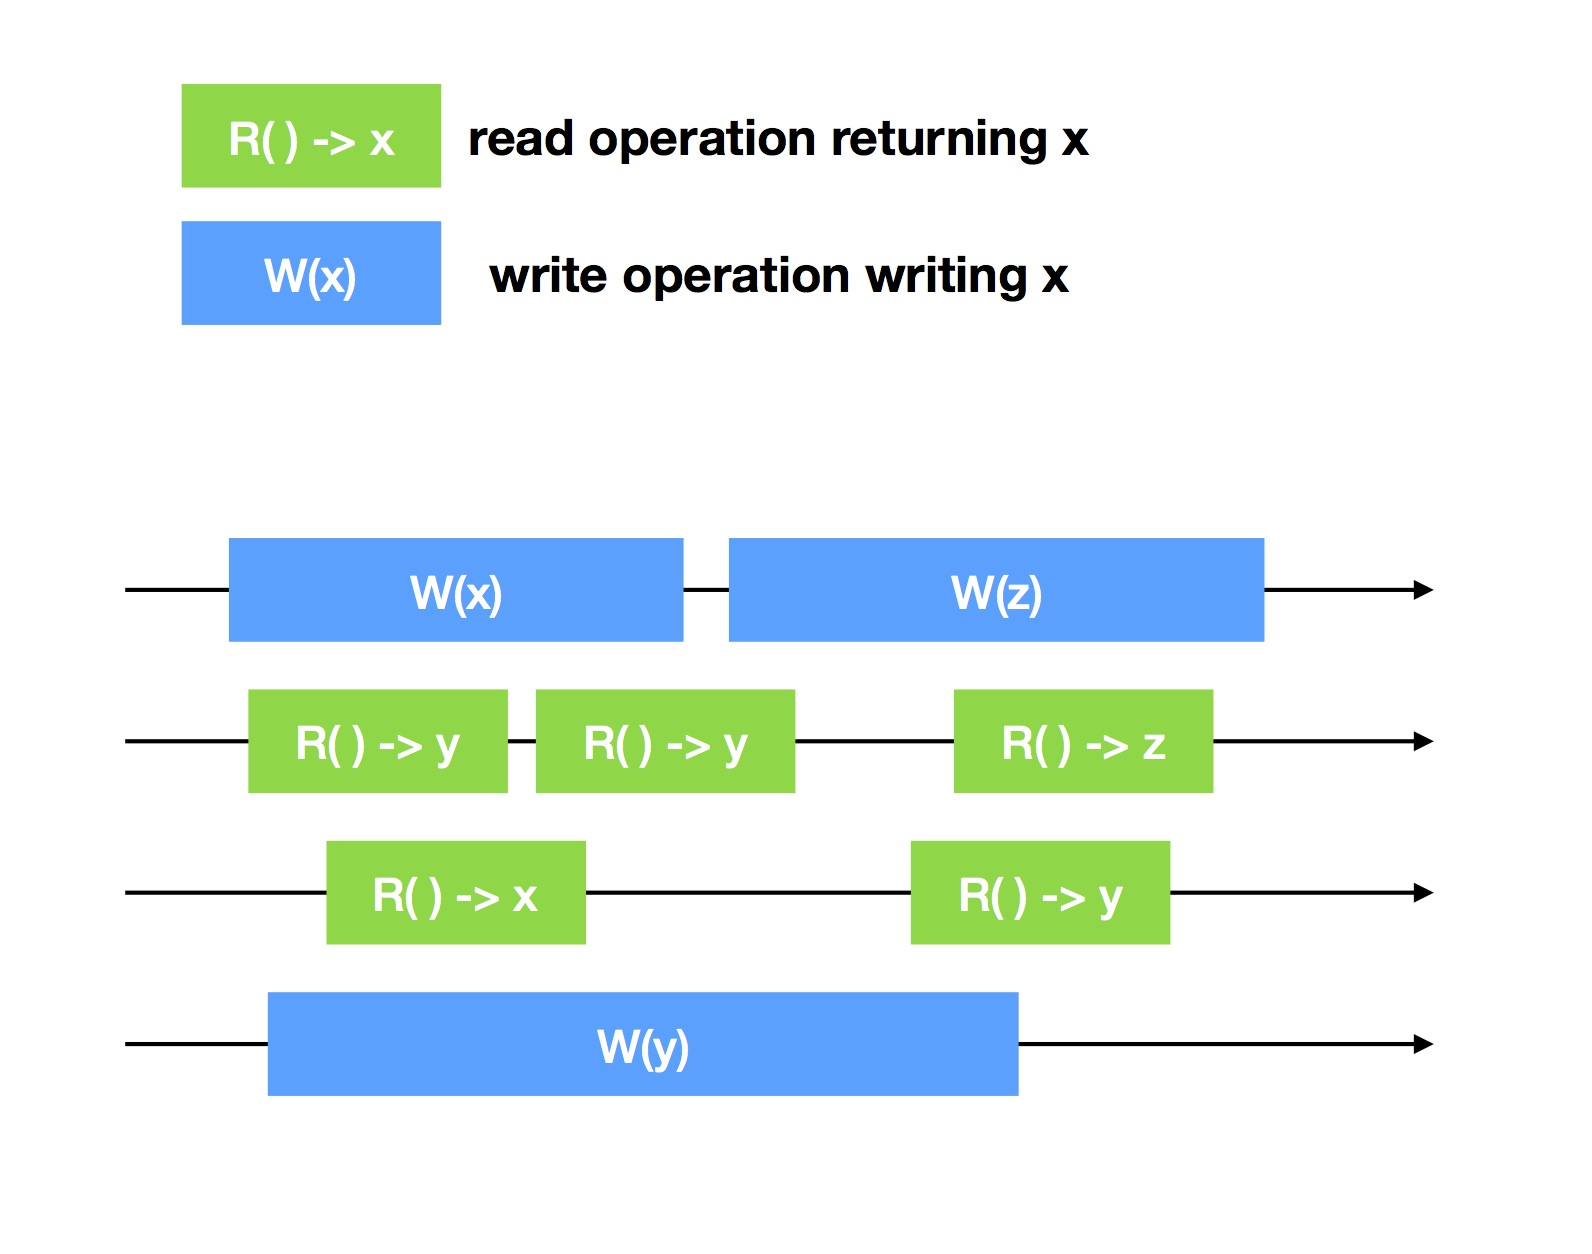
\includegraphics[width=\linewidth]{fig/RegisterOperations}
    \caption{Figure taken from~\cite{lecture}}
    \label{fig:example}
\end{figure}

You can create graphs from your experiment-data using \texttt{pgfplots}.
See the example in \texttt{tex/evaluation.tex} and documentation \url{http://pgfplots.sourceforge.net/pgfplots.pdf}.

\subsection{Other tips}
\begin{itemize}

\item Always use the tilde character between the number and unit, e.g. 100~Mbps or 53~ms. The tilde inserts a space, but prevents line break between the number and unit.

\item Never put SI units in italics. 

\item Do differentiate between bits (b) and bytes (B), and between powers of 10~(MB) and 2~(MiB).

\item Avoid things like: "We refer the reader to [42]." That is, don't use citations as nouns.
\end{itemize}

For further instructions on how to add \textbf{Tables, Algorithms, Theorems see acmguide.pdf}.


\section{Further Reading}
\label{sec:further}
Here are some other useful resources: (make these into references instead of links?)
\begin{itemize}
\item The co-chairs of the Ninth SOSP prepared some recommendations and valuable lessons in a paper titled \textit{How (and How Not) to Write a Good Systems Paper} \url{https://www.usenix.org/legacy/publications/library/proceedings/dsl97/good_paper.html}
\item \url{http://gramoli.redbellyblockchain.io/web/doc/talks/researchmethod.pdf}
\item \url{https://www.doc.ic.ac.uk/~prp/doc/talks/11-prp-paper_writing.pdf}
\item This template is inspired by a template from Markus P\"uschel~\cite{puschel}.

\end{itemize}

\bibliographystyle{ACM-Reference-Format}
\bibliography{sample-bibliography}

\end{document}
